\documentclass[12pt]{report}
\usepackage[utf8]{inputenc}
\usepackage[russian]{babel}
%\usepackage[14pt]{extsizes}
\usepackage{listings}
\usepackage{graphicx}
\usepackage{amsmath,amsfonts,amssymb,amsthm,mathtools} 
\usepackage{pgfplots}
\usepackage{filecontents}
\usepackage{float}
\usepackage{indentfirst}
\usepackage{eucal}
\usepackage{enumitem}
%s\documentclass[openany]{book}
\frenchspacing

\usepackage{indentfirst} % Красная строка

\usetikzlibrary{datavisualization}
\usetikzlibrary{datavisualization.formats.functions}

\usepackage{amsmath}


% Для листинга кода:
\lstset{ %
	language=c,                 % выбор языка для подсветки (здесь это С)
	basicstyle=\small\sffamily, % размер и начертание шрифта для подсветки кода
	numbers=left,               % где поставить нумерацию строк (слева\справа)
	numberstyle=\tiny,           % размер шрифта для номеров строк
	stepnumber=1,                   % размер шага между двумя номерами строк
	numbersep=5pt,                % как далеко отстоят номера строк от подсвечиваемого кода
	showspaces=false,            % показывать или нет пробелы специальными отступами
	showstringspaces=false,      % показывать или нет пробелы в строках
	showtabs=false,             % показывать или нет табуляцию в строках
	frame=single,              % рисовать рамку вокруг кода
	tabsize=2,                 % размер табуляции по умолчанию равен 2 пробелам
	captionpos=t,              % позиция заголовка вверху [t] или внизу [b] 
	breaklines=true,           % автоматически переносить строки (да\нет)
	breakatwhitespace=false, % переносить строки только если есть пробел
	escapeinside={\#*}{*)}   % если нужно добавить комментарии в коде
}


\usepackage[left=2cm,right=2cm, top=2cm,bottom=2cm,bindingoffset=0cm]{geometry}
% Для измененных титулов глав:
\usepackage{titlesec, blindtext, color} % подключаем нужные пакеты
\definecolor{gray75}{gray}{0.25} % определяем цвет
\newcommand{\hsp}{\hspace{20pt}} % длина линии в 20pt
% titleformat определяет стиль
\titleformat{\chapter}[hang]{\Huge\bfseries}{\thechapter\hsp\textcolor{gray75}{|}\hsp}{0pt}{\Huge\bfseries}


% plot
\usepackage{pgfplots}
\usepackage{filecontents}
\usetikzlibrary{datavisualization}
\usetikzlibrary{datavisualization.formats.functions}

\begin{document}

	\thispagestyle{empty}
\begin{titlepage}

\noindent \begin{minipage}{0.15\textwidth}
	
\includegraphics[width=\linewidth]{img/b_logo}
	\end{minipage}
	\noindent\begin{minipage}{0.9\textwidth}\centering
		\textbf{Министерство науки и высшего образования Российской Федерации}\\
		\textbf{Федеральное государственное бюджетное образовательное учреждение высшего образования}\\
		\textbf{~~~«Московский государственный технический университет имени Н.Э.~Баумана}\\
		\textbf{(национальный исследовательский университет)»}\\
		\textbf{(МГТУ им. Н.Э.~Баумана)}
	\end{minipage}
	
	\noindent\rule{18cm}{3pt}
	\newline\newline
	\noindent ФАКУЛЬТЕТ $\underline{\text{~~~~~~~~~~~~~~~~~~~«Информатика и системы управления»~~~~~~~~~~~~~~}}$ \newline\newline
	\noindent КАФЕДРА $\underline{\text{«Программное обеспечение ЭВМ и информационные технологии»}}$\newline\newline\newline\newline\newline
	
	\begin{center}
		\noindent\begin{minipage}{1.1\textwidth}\centering
			\Large\textbf{  Отчет по лабораторной работе №2}\newline
			\textbf{по дисциплине <<Математическая статистика>>}\newline\newline
		\end{minipage}
	\end{center}
	
	\noindent\textbf{Тема} $\underline{\text{~~~~~~~~~~~~~~~~~~~~~~~~~~~~~~~Интервальные оценки~~~~~~~~~~~~~~~~~~~~~~~~~~~~~~~~~~~~~~~~~~~~~~~~~~~~~~~}}$\newline\newline
	\noindent\textbf{Группа} $\underline{\text{~~~~~~~~~~~~~~~~~~~~~~~~~~~~~~~~~~~~ИУ7-63Б~~~~~~~~~~~~~~~~~~~~~~~~~~~~~~~~~~~~~~~~~~~~~~~~~~~~~~~~~~~~~~~~~}}$\newline\newline
	\noindent\textbf{Студент} $\underline{\text{~~~~~~~~~~~~~~~~~~~~~~~~~~~~~~~~Сукочева А.~~~~~~~~~~~~~~~~~~~~~~~~~~~~~~~~~~~~~~~~~~~~~~~~~~~~~~~~~~~~~~}}$\newline\newline
	\noindent\textbf{Преподаватель} $\underline{\text{~~~~~~~~~~~~~~~~~~~~~Саркисян П.С.~~~~~~~~~~~~~~~~~~~~~~~~~~~~~~~~~~~~~~~~~~~~~~~~~~~~~~~~~~~}}$\newline\newline\newline
	
\begin{center}
	\vfill
	Москва~---~\the\year
	~г.
\end{center}

\end{titlepage}

	\chapter{Задание}

	\section{Цель работы}

	\textbf{Цель работы:} построение гистограммы и эмпирической функции распределения.

	\section{Содержание работы}

	\begin{enumerate}
		\item Для выборки объёма $n$ из генеральной совокупности $X$ реализовать в виде программы на ЭВМ
			\begin{enumerate}
				\item вычисление максимального значения $M_{\max}$ и минимального значения $M_{\min}$;
				\item размаха $R$ выборки;
				\item вычисление оценок $\hat\mu$ и $S^2$ математического ожидания $MX$ и дисперсии $DX$;
				\item группировку значений выборки в $m = [\log_2 n] + 2$ интервала;
				\item построение на одной координатной плоскости гистограммы и графика функции плотности распределения вероятностей нормальной случайной величины с математическим ожиданием $\hat{\mu}$ и дисперсией $S^2$;
				\item построение на другой координатной плоскости графика эмпирической функции распределения и функции распределения нормальной случайной величины с математическим ожиданием $\hat{\mu}$ и дисперсией $S^2$.
			\end{enumerate}
		\item Провести вычисления и построить графики для выборки из индивидуального варианта.
	\end{enumerate}

\chapter{Теоретическая часть}

\section{Формулы для вычисления величин}

\subsection{Минимальное и максимальное значения выборки}
\begin{equation}
    \begin{aligned}
        M_{\max} = X_{(n)}\\
        M_{\min} = X_{(1)}
    \end{aligned}
\end{equation}

\subsection{Размах выборки}
\begin{equation}
    R = M_{\max} - M_{\min}.
\end{equation}

\subsection{Оценки математического ожидания и дисперсии}
\begin{equation}
    \begin{aligned}
    \hat\mu(\vec X_n) &= \frac 1n \sum_{i=1}^n X_i\\
    S^2(\vec X_n) &= \frac 1{n-1} \sum_{i=1}^n (X_i-\overline X_n)^2
    \end{aligned}
\end{equation}

\section{Эмпирическая плотность и гистограмма}

Пусть 

$\vec x$ -- выборка из генеральной совокупности $X$. 

При большом объеме n этой выборки  значения $x_i$ группируют в интервальный статистический ряд. 

Отрезок $J = [x_{(1)}, x_{(n)}]$ делят на $m$ равновеликих частей:

\begin{equation}
    J_i = [x_{(1)} + (i - 1) \cdot \Delta, x_{(1)} + i \cdot \Delta), i = \overline{1; m - 1}
\end{equation}

\begin{equation}
    J_{m} = [x_{(1)} + (m - 1) \cdot \Delta, x_{(n)}]
\end{equation}

\begin{equation}
    \Delta = \frac{|J|}{m} = \frac{x_{(n)} - x_{(1)}}{m}
\end{equation}

\newpage

\textbf{Интервальным статистическим рядом называют таблицу:}

\begin{table}[htb]
    \centering
    \begin{tabular}{|c|c|c|c|c|}
        \hline
        $J_1$ & ... & $J_i$ & ... & $J_m$ \\
        \hline
        $n_1$ & ... & $n_i$ & ... & $n_m$ \\
        \hline
    \end{tabular}
\end{table}

где $n_i$ -- количество элементов выборки $\vec x$, которые $\in J_i$.

% Обычно выборку разбивают на $m=[\log_2n]+2$ интервалов, где $n$ -- размер выборки.

\textbf{Гистограмма} -- это график эмпирической плотности. 

\textbf{Эмпирической плотностью}, отвечающей выборке $\vec x$, называют функцию:
\begin{equation}
    \hat f(x) =
    \begin{cases}
        \frac{n_i}{n \Delta}, x \in J_i, i = \overline{1; m} \\
        0, \text{иначе} \\
    \end{cases}
\end{equation}

где $J_i$ -- полуинтервал статистического ряда, 
$n_i$ -- количество элементов выборки, входящих в полуинтервал, 
$n$ -- количество элементов выборки.


\section{Эмпирическаяя функция распределения}

Пусть $\vec x = (x_1, ..., x_n)$ -- выборка из генеральной совокупности $X$. 

Обозначим $n(x, \vec x)$ -- число элементов вектора $\vec x$, которые имеют значения меньше $x$.

\textbf{Эмпирической функцией распределения} называют функцию $F_n: \mathbb{R} \to \mathbb{R}$, определенную как: 

\begin{equation}
    F_n(x) = \frac{n(x, \vec x)}{n}
\end{equation}

\chapter{Практическая часть}

\begin{figure}[ht!]	
	\centering{
		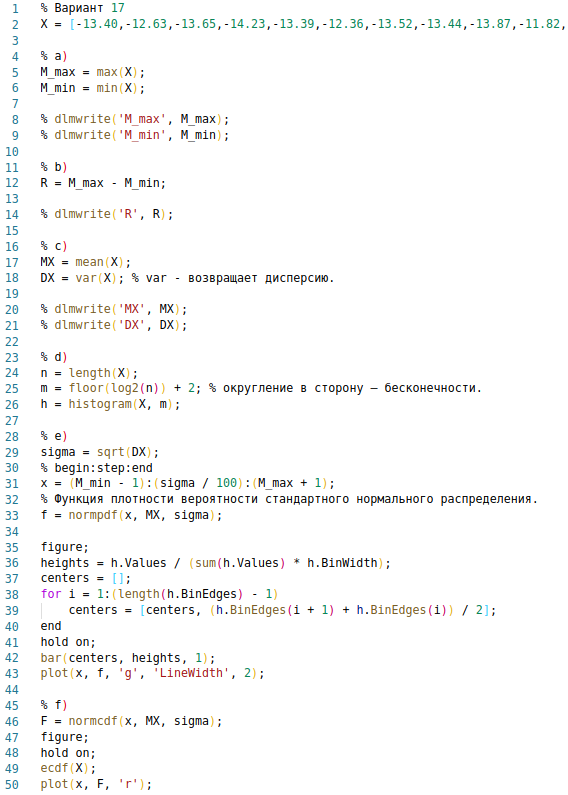
\includegraphics[width=0.75\textwidth]{img/code.png}}
\end{figure}

\chapter{Экспериментальная часть}

\section{Результаты расчетов}

\begin{figure}[ht!]	
	\centering{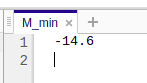
\includegraphics[width=0.25\textwidth]{img/res1.png}}
\end{figure}


\begin{figure}[ht!]	
	\centering{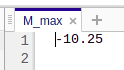
\includegraphics[width=0.25\textwidth]{img/res2.png}}
\end{figure}

\begin{figure}[ht!]	
	\centering{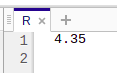
\includegraphics[width=0.25\textwidth]{img/res5.png}}
\end{figure}

\begin{figure}[ht!]	
	\centering{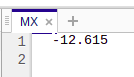
\includegraphics[width=0.25\textwidth]{img/res3.png}}
\end{figure}


\begin{figure}[ht!]	
	\centering{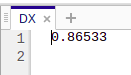
\includegraphics[width=0.25\textwidth]{img/res4.png}}
\end{figure}

\begin{figure}[ht!]	
	\centering{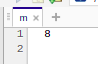
\includegraphics[width=0.25\textwidth]{img/res6.png}}
\end{figure}

\begin{figure}[ht!]	
	\centering{
		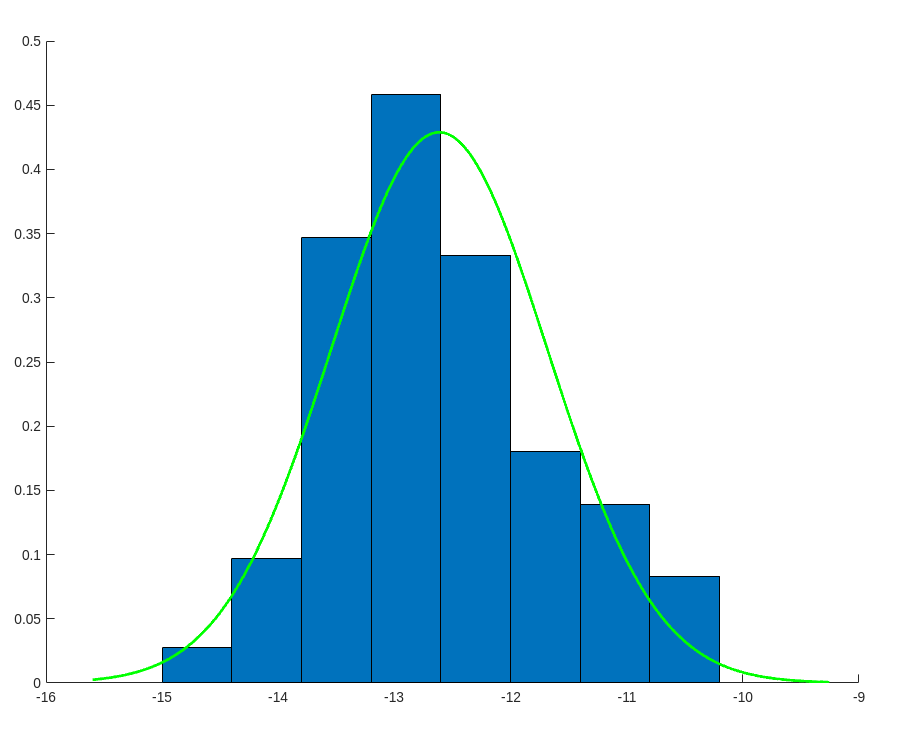
\includegraphics[width=0.6\textwidth]{img/1.png}
		\caption{Гистограмма и график функции плотности распределения вероятностей нормальной случайной величины с выборочными мат. ожиданием и дисперсией}}
\end{figure}

\begin{figure}[ht!]	
	\centering{
		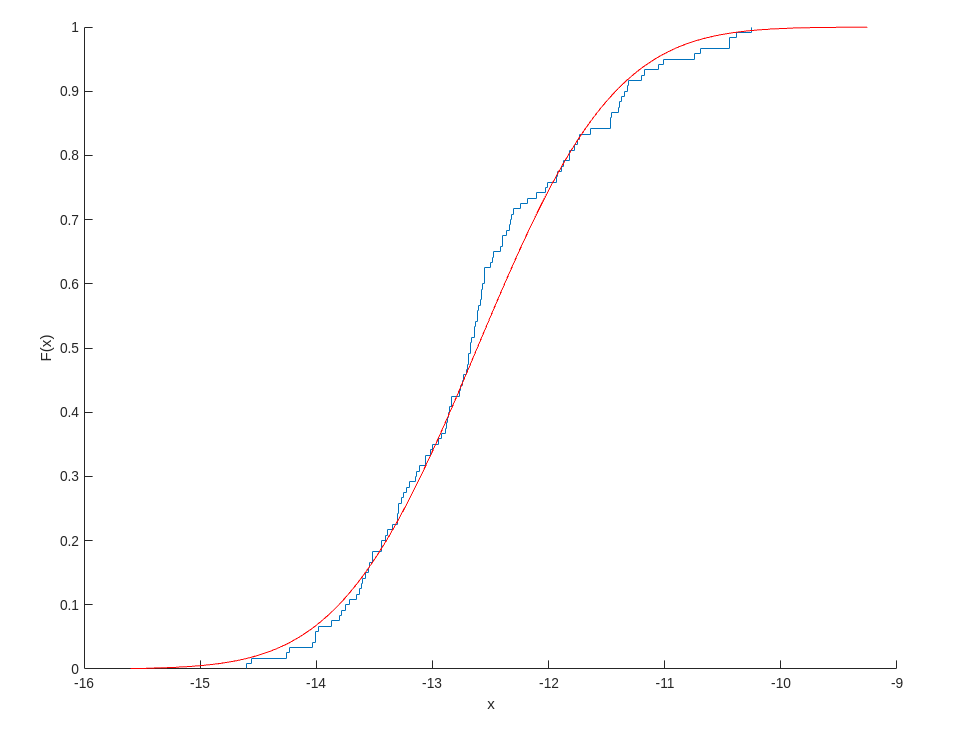
\includegraphics[width=0.6\textwidth]{img/2.png}
		\caption{График эмперической функции распределения и функции распределения нормальной случайной величины с выборочными мат. ожиданием и дисперсией}}
\end{figure}

\end{document}
